\chapter{Project Development}
	
In each of the previous chapters I have explored different aspects of the fields of home automation and voice assistance from a 
theoretical point of view, from their definition to smaller details, including additional explanations about a specific home automation 
system, openHAB.

At this time, I think I have provided enough background to begin my case study: the building of a home automation controller. As I 
mentioned in the openHAB chapter, I will base my project on this system and build on it, as it accomplishes very well the main
requirements that I determined for this project.

In this chapter, I will detail the process that I have followed in order to develop this project, from its specification to the final result.

\section{Product Specification}
The first task to do is to define the product. What should a home automation system do? What do users expect it to do? How? All 
the answers to these questions can be clarified by following some processes that, although they do not completely answer them (we 
can see many failed projects from time to time), they provide a very clear and detailed specification from the beginning.

\subsection{Personas}
Creating personas is a common process applied to the product design and development process in order to help in making a user-centered
design, and it is applicable in this project in order to have a better idea of what would users expect from the final product.

A persona is a representation of a user, typically based off user research and incorporating user goals, needs, and interests.

In this project, I am going to use proto-personas, which are based on secondary research and the guess of who they should be designed 
for, as currently we do not have means and time for making true research-based personas (and it is not the main objective in this project).

After thinking about the main uses of this system and the people that would be interested on it, I have extracted these three personas, 
representing its main uses, although not the only ones. I have built them with the online platform Xtensio, and the figures
\ref{fig:persona-oswald-douglas}, \ref{fig:persona-anna-lahtinen} and \ref{fig:persona-rosario-vera} represent them.

I tried to extract a varied range of backgrounds, current situations, desires and worries. Oswald Douglas (figure 
\ref{fig:persona-oswald-douglas}) is a freelance technology blogger from Dallas, USA, that is very interested in the areas of home 
automation and Internet of Things. He is looking to automate his own home and write about his experience in his blog. He already has 
experience with technology, and this next step will not be too difficult for him. His interests are clear: to try cutting-edge technology 
in his own home and make the most of home automation.

Anna Lahtinen is a 16 year-old high school student from Lappeenranta, Finland. She is up to date on technology but she is not passionate 
about it. However, she heard about home automation and thinks that she could enjoy a better media experience with it. In addition, she 
thinks that adding smart color light bulbs to her bedroom would make it look more beautiful. However, she feels that there is a lack
of general information about devices and the set up and configuration of a home automation system. She thinks that the price
of it is too high as well.

Rosario Vera is an administrative from Vitoria-Gasteiz, Spain. She is 37 years old, is married and has two young children. She is not 
very familiar with technology, but she has heard about home automation in the news and thinks that it could fit her needs. Rosario
and her husband work outside home, and sometimes their children need to be alone at home. Home automation would provide more security
to the home and would allow them to have more spare time. Voice assistance would be helpful for their children when they are alone,
as it is a very easy and natural way to interact with technology. However, she is concerned about their privacy regarding these systems
and she thinks that companies should give more accessible explanations about it. In addition, she finds these systems difficult to use.

\begin{sidewaysfigure}
	\centering
	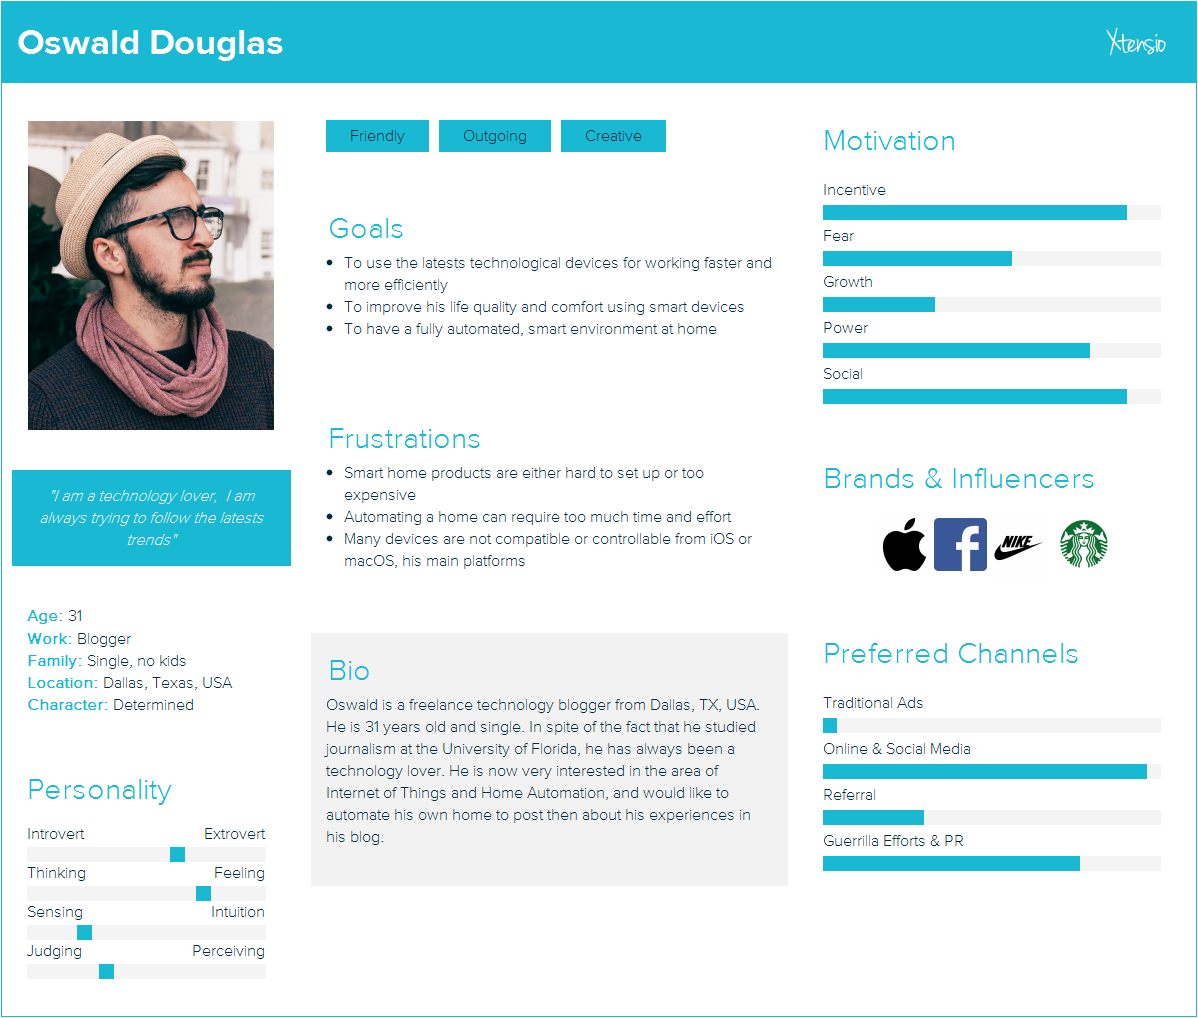
\includegraphics[width=0.65\textwidth]{images/Chapter_06/persona-oswald-douglas.png}
	\caption{Persona: Oswald Douglas}
	\label{fig:persona-oswald-douglas}
\end{sidewaysfigure}

\begin{sidewaysfigure}
	\centering
	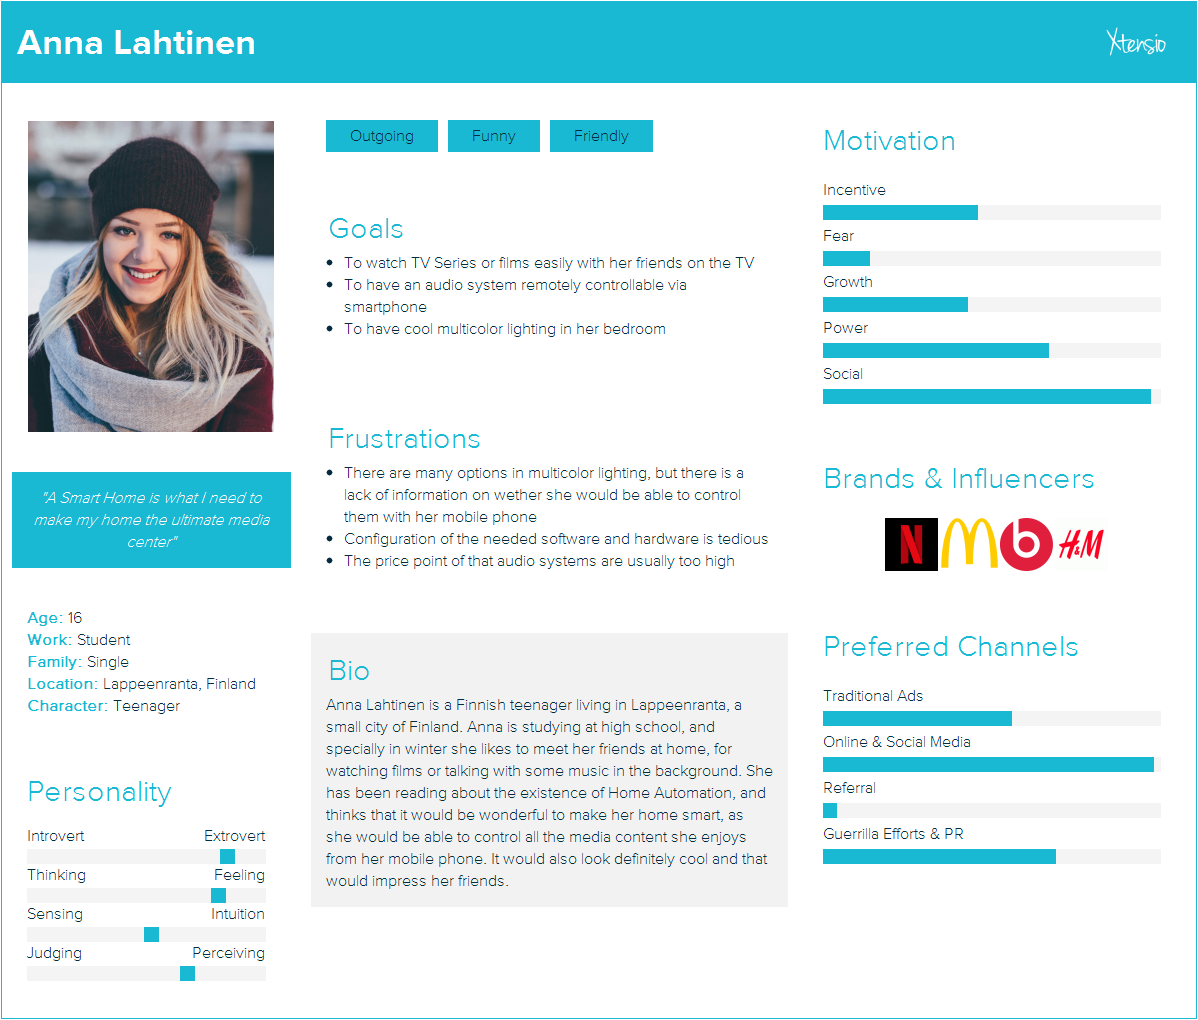
\includegraphics[width=0.65\textwidth]{images/Chapter_06/persona-anna-lahtinen.png}
	\caption{Persona: Anna Lahtinen}
	\label{fig:persona-anna-lahtinen}
\end{sidewaysfigure}

\begin{sidewaysfigure}
	\centering
	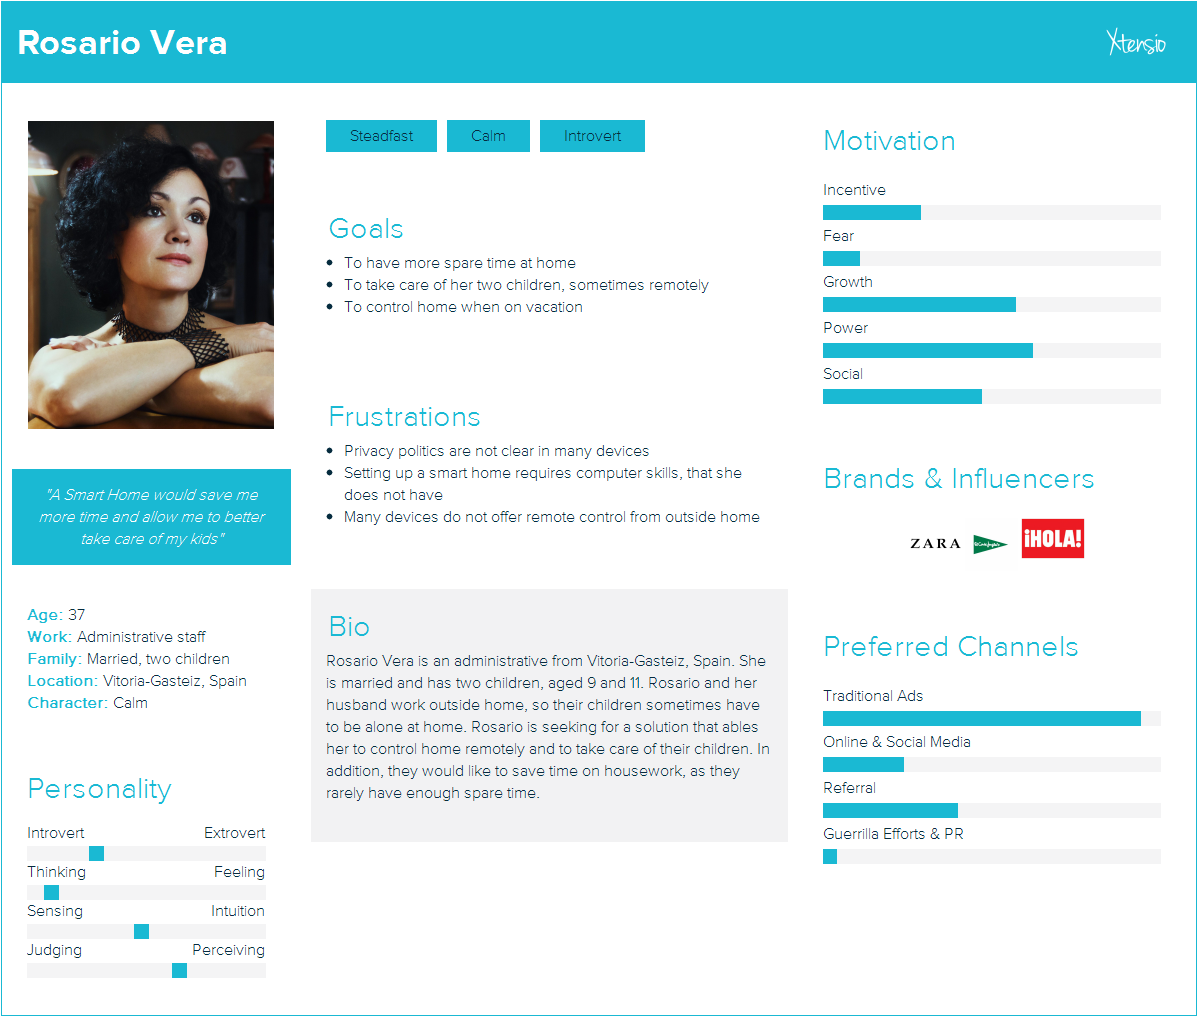
\includegraphics[width=0.65\textwidth]{images/Chapter_06/persona-rosario-vera.png}
	\caption{Persona: Rosario Vera}
	\label{fig:persona-rosario-vera}
\end{sidewaysfigure}

\subsection{Software Requirements Specification}
With the Software Requirements Specification (SRS), I try to describe the project to develop from a functional point of view, that is,
to determine the capabilities that the software system will have.
